\documentclass[conference]{IEEEtran}
\IEEEoverridecommandlockouts
\usepackage{cite}
\usepackage{amsmath,amssymb,amsfonts}
\usepackage{algorithmic}
\usepackage{graphicx}
\usepackage{textcomp}
\usepackage{xcolor}
\usepackage[utf8]{inputenc}
\usepackage{booktabs}
\usepackage{float}
\usepackage[portuguese]{babel}

\makeatletter
\newcommand{\linebreakand}{%
\end{@IEEEauthorhalign}
\hfill\mbox{}\par
\mbox{}\hfill\begin{@IEEEauthorhalign}
}
\makeatother

\def\BibTeX{{\rm B\kern-.05em{\sc i\kern-.025em b}\kern-.08em
		T\kern-.1667em\lower.7ex\hbox{E}\kern-.125emX}}

\begin{document}

\title{ANADI - Trabalho Prático 2:\\
Análise de Desempenho De Técnicas de Aprendizagem Automática}

\author{\IEEEauthorblockN{Fábio Borges\IEEEauthorrefmark{1}, Joel Ferreira\IEEEauthorrefmark{2}, Jorge Cruz\IEEEauthorrefmark{3}}
\IEEEauthorblockA{\textit{Departamento de Engenharia Informática}} \\
\textit{Instituto Superior de Engenharia do Porto}\\
Porto, Portugal \\
\IEEEauthorrefmark{1} 1100719@isep.ipp.pt\\
\IEEEauthorrefmark{2} 1191843@isep.ipp.pt\\
\IEEEauthorrefmark{3} 1221715@isep.ipp.pt\\
}


\maketitle

\begin{abstract}
Este artigo tem como objetivo a aplicação de algoritmos de aprendizagem automática na exploração de dados e respetiva comparação usando os testes estatísticos mais adequados. A temática incide sobre os níveis de poluição e seus impactos em diversos países europeus, no âmbito da disciplina de Análise de Dados em Informática. 

\textcolor{red}{É verificado se os dados são estatisticamente válidos e se se podem tirar conclusões dos mesmo, nomeadamente relações entre países e doenças, mas também de mortes prematuras associadas aos diferentes níveis médios de poluição.  }
\end{abstract}

\begin{IEEEkeywords}
poluição, saúde, regressão linear, árvores de decisão, K-vizinhos-mais-próximos, redes neuronais, SVM
\end{IEEEkeywords}

\section{Introdução}

Este artigo começa por fazer uma introdução aos conceitos teóricos relevantes para a execução do trabalho e que foram abordados na disciplina de ANADI, \textbf{nomeadamente distribuição de dados, testes, correlações, regressões e previsões. }

De seguida, na ótica dos dados do problema - a poluição, são descritos os métodos e resultados obtidos em cada problema proposto. 

Por último, são apresentadas as conclusões do  trabalho.

Foi utilizado o \textit{python} para tratamento e processamento dos dados.

\section{Introdução Teórica}

Nesta secção serão introduzidos os conceitos teóricos sobre os diferentes algoritmos e modelos desenvolvidos na resolução deste trabalho. 

\subsection{Regressão}

\subsubsection{Regressão linear}

%\paragraph{}

A regressão linear é uma técnica estatística usada para modelar a relação entre uma variável dependente e uma ou mais variáveis independentes. Quando há apenas uma variável explicativa, o modelo é denominado \textbf{regressão linear simples}, sendo representado pela equação:

\begin{equation}
	Y = \beta_0 + \beta_1 X + \varepsilon
\end{equation}

onde \( Y \) é a variável que tentamos prever, denominada variável dependente. \( X \) é a variável independente (ou preditora), \( \beta_0 \) e \( \beta_1 \) são os coeficientes do modelo, e \( \varepsilon \) representa o erro aleatório. \cite{madureira2024aed}

\subsubsection{Regressão linear múltipla}
A regressão linear múltipla é uma extensão da regressão linear simples, na qual há mais de uma variável independente. A equação do modelo assume a forma:

\begin{equation}
	Y = \beta_0 + \beta_1 X_1 + \beta_2 X_2 + \dots + \beta_n X_n + \varepsilon
\end{equation}

Para se poder aplicar a regressão linear múltipla é necessário que exista uma relação linear entre a variável objetivo (Y) e as variáveis preditoras, os resíduos da regressão devem seguir uma distribuição normal e não deve existir multicolineariadade.\cite{madureira2024aed}

\subsection{Métricas de avaliação de modelos de regressão}

As métricas MAE, MSE, RMSE e R$^2$ são utilizadas principalmente para avaliar as taxas de erro de previsão e o desempenho do modelo na análise de regressão.

\medskip
\subsubsection{Mean Absolute Error - MAE}
Erro absoluto médio, é a soma das diferenças absolutas entre as previsões e os valores reais, dividindo pelo número total de pontos de dados.


\begin{equation}
	MAE = \frac{1}{n} {\sum_{i=1}^{n} |y_i - \hat{y_i}|}
	 \label{MAEeq}
\end{equation}

\medskip
\subsubsection{Mean Squared Error - MSE}
Erro quadrático médio, representa a diferença entre os valores originais e os valores previstos extraídos através do quadrado da diferença média do conjunto de dados.

\medskip
\subsubsection{Root Mean Squared Error - RMSE}
Mede a magnitude média do erro, tomando a raiz quadrada da média das diferenças quadráticas entre a previsão ($\hat{y_i}$) e a observação efetiva ($y_i$).


\begin{equation}
	RMSE = \sqrt{\frac{1}{n} {\sum_{i=1}^{n} (y_i - \hat{y_i})^2}}
	\label{RMSEeq}
\end{equation}

O RMSE é uma boa medida de exatidão, mas apenas para comparar erros de previsão de diferentes modelos ou configurações de modelos para uma determinada variável e não entre variáveis, uma vez que é dependente da escala. 

\medskip
\subsubsection{R$^2$ - Coeficiente de Determinação}

Representa o coeficiente de determinação dos valores em comparação com os valores originais. O valor de 0 a 1 é interpretado como percentagem. Quanto mais elevado for o valor, melhor é o modelo.\cite{madureira2024cv} 


\subsection{Correlação}
Em estatística, a correlação é uma medida que indica o grau de associação entre duas variáveis. Ela quantifica a intensidade e a direção da relação linear entre as variáveis.
 A correlação é sempre um número entre -1 e 1. Valores próximos de 0 indicam uma relação linear muito fraca. A força da relação aumenta à medida que esta se afasta de 0 em direção a -1 ou 1. Valores próximos de -1 ou 1 indicam que os pontos estão próximos duma linha reta. Os valores extremos -1 e 1 ocorrem apenas quando os pontos de um gráfico de dispersão se encontram  exatamente ao longo de uma linha reta. \cite{moore2017}

\medskip
\subsubsection{Testes de Correlação}

\paragraph{Pearson}

O coeficiente de correlação mais comum é o Coeficiente de Correlação de Pearson (r), que varia entre -1 e 1. Para aplicar o teste \eqref{pearsonEq}, é necessário cumprir quatro pressupostos \cite{madureira2024}:

\begin{itemize}
	\item As variáveis devem ser contínuas e não devem existir \textit{outliers} significativos.
	\item Deve existir uma relação linear entre as duas variáveis.
	\item As variáveis devem ter aproximadamente uma distribuição normal.
	\item Variâncias iguais (Homocedasticidade).

\end{itemize}

\begin{equation}
r = \frac{\sum_{i=1}^{n} (x_i - \bar{x})(y_i - \bar{y})}
{\sqrt{\sum_{i=1}^{n} (x_i - \bar{x})^2 \sum_{i=1}^{n} (y_i - \bar{y})^2}} \label{pearsonEq}
\end{equation}

cujas hipóteses são:
\begin{itemize}
\item Hipótese nula ($H_0$): Não há correlação linear significativa entre as variáveis (r = 0).
\item Hipótese alternativa ($H_1$): Existe correlação linear significativa entre as variáveis (r $\neq$ 0).
\end{itemize}

\medskip
\paragraph{Spearman}

Este teste é usado quando as variáveis são ambas ordinais ou quando uma das variáveis é contínua e a outra é ordinal \cite{madureira2024}.

De forma semelhante, o coeficiente de Spearman ($\rho$) avalia a correlação entre -1 e 1, resultado obtido da aplicação da fórmula:

\begin{equation}
	\label{eq:spearman}
	\rho = 1 - \frac{6 \sum_{i=1}^n d_i^2}{n(n^2-1)}
\end{equation}

Onde:
\begin{itemize}

\item $d_i$ é a diferença entre os postos (ranks) das observações correspondentes nas duas variáveis,

\item \textit{n} é o número total de observações \cite{zar2005}.

\end{itemize}

\subsection{Árvores de Decisão}

Uma árvore de decisão,  \figurename~\ref{fig:Decision_Trees_example},  consiste num conjunto de nós de decisão, ligados por ramos, que se estendem para baixo a partir do nó raiz até terminarem em nós folha. 

Começando no nó raiz, que por convenção é colocado no topo do diagrama de árvore de decisão, as variáveis são testadas nos nós de decisão, sendo que cada resultado possível resulta num ramo. Cada ramo conduz então a outro nó de decisão ou a um nó folha terminal. 

A aprendizagem em árvore de decisão é um método de aproximação de uma função-alvo de valor discreto representada numa árvore de decisão. \cite{madureira2024dt}

\begin{figure}[h]
	\centering
	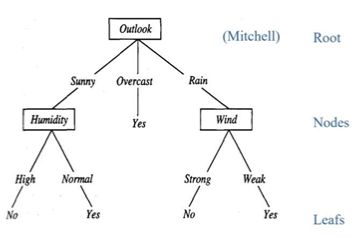
\includegraphics[width=0.9\linewidth]{Decision_Trees_example}
	\caption{Exemplo de árvore de decisão. \cite{madureira2024dt}}
	\label{fig:Decision_Trees_example}
\end{figure}

\subsubsection{Árvore de Decisão - Regressão}

As árvores de regressão são utilizados para prever variáveis-alvo contínuas, como o preço de uma casa ou o número de clientes que visitarão uma loja num determinado dia. Para fazer uma previsão, o regressor da árvore de decisão percorre a árvore desde o nó raiz até ao nó folha que corresponde às caraterísticas do novo ponto de dados. O valor previsto é então o valor médio da variável alvo para todos os pontos de dados no nó folha. \cite{ohekar_what_2023}

\medskip
\subsubsection{Árvore de Decisão - Classificação}

Os classificadores de árvores de decisão são utilizados para prever variáveis-alvo categóricas, como, por exemplo, se uma mensagem de correio eletrónico é ou não spam ou se um cliente vai ou não desistir. Para efetuar uma previsão, o classificador de árvore de decisão percorre a árvore desde o nó raiz até ao nó folha que corresponde às caraterísticas do novo ponto de dados. A classe prevista é então a classe com a maioria dos pontos de dados no nó folha. \cite{ohekar_what_2023}

\subsection{Cross-Validation}

A validação cruzada (Cross-Validation) é um método estatístico de avaliação e comparação de algoritmos de aprendizagem, dividindo os dados em dois segmentos: um utilizado para treinar um modelo e o outro utilizado para validar o modelo. Na validação cruzada típica, os conjuntos de treino e validação devem cruzar-se em rondas sucessivas, de modo a que cada ponto de dados tenha uma hipótese de ser validado. \cite{refaeilzadeh_cross-validation_2009}

\medskip
\subsubsection{Hold Out}

Esta abordagem consiste em dividir aleatoriamente os dados em dois conjuntos: um conjunto é utilizado para treinar o modelo e o outro conjunto é utilizado para testar o modelo. O processo funciona da seguinte forma: 
\begin{itemize}
	\item Construir (treinar) o modelo no conjunto de dados de treino; 
	\item Aplicar o modelo ao conjunto de dados de teste para prever o resultado de novas observações não vistas; 
	\item Quantificar o erro de previsão como a diferença média quadrática entre os valores de resultados observados e previstos.
\end{itemize}

\medskip
\subsubsection{K-Fold Cross-Validation}

O método de validação cruzada \textit{k-fold} avalia o desempenho do modelo em diferentes subconjuntos dos dados de treino e, em seguida, calcula a taxa média de erro de previsão. O algoritmo é o seguinte:
\begin{enumerate}
	\item Dividir aleatoriamente o conjunto de dados em \textit{k} subconjuntos (ou \textit{k-fold}) (por exemplo, 5 subconjuntos);
	\item Reservar um subconjunto e treinar o modelo em todos os outros subconjuntos;
	\item Testar o modelo no subconjunto reservado e registar o erro de previsão;
	\item Repetir este processo até que cada um dos \textit{k} subconjuntos tenha servido como conjunto de teste; 
	\item Calcular a média dos \textit{k} erros registados. Este é o chamado erro de validação cruzada, que serve de métrica de desempenho para o modelo. 
\end{enumerate}

A validação cruzada \textit{K-fold} (CV) é um método robusto para estimar a exatidão de um modelo. \cite{madureira2024cv}

\subsection{Redes Neuronais}

Uma rede neuronal, \figurename~\ref{fig:nn}, consiste numa rede de neurónios artificiais ou nós, em camadas, com alimentação direta e completamente ligada:

\begin{itemize}
	\item A natureza \textit{feedforward} da rede restringe-a uma única direção de fluxo e não permite ciclos. 
	\item A maioria das redes é constituída por três camadas: uma camada de entrada, uma camada oculta e uma camada de saída; 
	\begin{itemize}
		\item Pode haver mais de uma camada oculta, embora a maioria das redes contenha apenas uma, o que é suficiente para a maioria das finalidades.
	\end{itemize}
	
	  
	\item  A rede neuronal está completamente ligada, o que significa que cada nó de uma determinada camada está ligado a todos os nós das camadas adjacentes, mas não a outros nós da mesma camada:
	\begin{itemize}
		\item Cada conexão entre nós tem um peso (por exemplo, $w_{11}$) associado.
		\item  Na inicialização, estes pesos são atribuídos aleatoriamente a valores entre 0 e 1.
	\end{itemize}
\end{itemize}

\begin{figure}
	\centering
	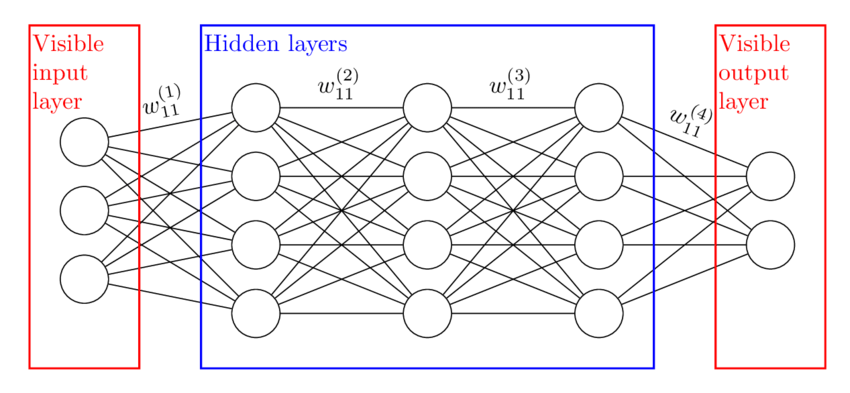
\includegraphics[width=0.9\linewidth]{NN}
	\caption{Exemplo de rede neuronal.}
	\label{fig:nn}
\end{figure}



\subsubsection{Regressão}

\subsubsection{Classificação}

\subsection{Support Vector Machines - SVM}


\section{Métodos e Resultados Obtidos}

\subsection{Análise Exploratória de Dados}
\medskip
\subsubsection{\textbf{Exercício 4.1.1}}

Neste exercício era pretendida a construção de um gráfico onde fosse possível verificar os níveis médios do poluente O$_3$ nas diversas regiões de Portugal. Era também requisito identificar a região com nível de O$_3$ mais elevado. Foram então importados os dados onde constava essa informação (ficheiro AIRPOL$\_$data).  

Para uma melhor visualização dos dados e para utilizarmos apenas os dados necessários, filtramos os mesmos. Assim, foram selecionados apenas os dados correspondentes a Portugal e cujo poluente em questão seja O$_3$. Verificamos a existência de alguns dados duplicados, o que nos levou à eliminação dos mesmos de modo a limpar o \textit{dataset}.
 
O gráfico obtido pode ser observado na \figurename~\ref{fig:nivelmedioo3}. É possível então verificar que todas as regiões apresentam um nível médio de O$_3$ situado entre os 80 e os 102.4 µg/m$^3$. A região com o maior valor médio de poluente é PT16H com um valor de 102.4 µg/m$^3$.


\medskip
\subsubsection{\textbf{Exercício 4.1.2}}

Pretendia-se a construção de um gráfico para comparação das distribuições dos níveis médios de PM2.5 em Portugal, Espanha, França e Itália. 

Inicialmente, os dados foram importados e filtrados. Como tal, foram selecionados apenas os dados correspondentes aos países mencionados anteriormente e cujo poluente em questão fosse PM2.5. Verificamos a existência de alguns dados duplicados, o que nos levou à eliminação dos mesmos de modo a limpar o dataset.

O gráfico obtido pode ser observado na \figurename~\ref{fig:niveismediospm25}. É possível então concluir o seguinte:

- Itália é o país que apresenta os valores mais elevados de PM2.5. Apresenta \textit{outliers} e uma grande dispersão de dados.

- Portugal e França apresentam níveis mais baixos de concentração de PM2.5. Estes dois países também apresentam a menor dispersão. França, apresenta um número de outliers mais elevado do que Portugal.

- Espanha, encontra-se entre os grupos de países mencionados anteriormente. A sua dispersão é superior à de Portugal e França.

\begin{figure}
	\centering
	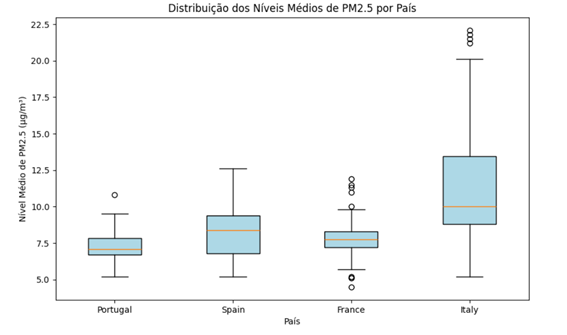
\includegraphics[width=0.9\linewidth]{Niveis_medios_pm25}
	\caption{Distribuição dos níveis médios de PM2.5 por País}
	\label{fig:niveismediospm25}
\end{figure}

\medskip
\subsubsection{\textbf{Exercício 4.1.3}}

O objetivo deste exercício consiste na construção de um gráfico para comparação do número de mortes prematuras entre Portugal, Espanha, França e Itália. 

Os dados foram importados e filtrados. Como tal, foram selecionados apenas os dados correspondentes aos países mencionados. Para melhor visualização do dataframe, selecionamos apenas as colunas correspondentes ao país e ao valor de mortes prematuras. 

O gráfico obtido pode ser observado na \figurename~\ref{fig:mortesprematuras}. É possível então concluir o seguinte:

- A média de mortes prematuras tende a seguir valores baixos, embora sejam visíveis \textit{outliers}.

- Itália destaca-se pelo país com os números mais extremos de mortes prematuras.

- Portugal é o país que apresenta menor dispersão e valores menores de mortes prematuras.


\begin{figure}
	\centering
	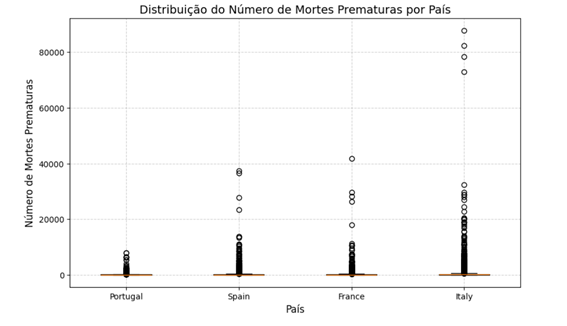
\includegraphics[width=0.9\linewidth]{mortes_prematuras}
	\caption{Distribuição do número de mortes prematuras por País}
	\label{fig:mortesprematuras}
\end{figure}


\medskip
\subsubsection{\textbf{Exercício 4.1.4}}

Neste exercício era pretendida a construção de uma tabela que indicasse os valores da média, quartis, desvio padrão, assimetria e \textit{Kurtosis} relativa ao número de mortes prematuras associadas a Stroke para os seguintes países: Espanha, França, Itália e Grécia. Foram então importados os dados onde constava essa informação (ficheiro AIRPOLdata). 
 
Para uma melhor visualização dos dados e para utilizarmos apenas os dados necessários, filtramos os mesmos. Assim, foram selecionados apenas os dados correspondentes aos países mencionados e cujas mortes prematuras estivessem associadas a AVC (Stroke). 

Da tabela apresentada na figura \figurename~\ref{fig:valoresestatisticos}, é possível concluir o seguinte:

- O valor da média varia entre os diferentes países. É notório que Itália regista o maior número de mortes prematuras por AVC. França regista a menor média.

- Relativamente aos quartis, Itália apresenta os valores mais elevados para os mesmos, reforçando a tendência para os valores elevados. Esta medida ajuda a entender a dispersão dos dados.

- Itália apresenta também o desvio-padrão mais elevado, o que prova mais uma vez a sua grande disperão de dados. França apresenta o menor desvio-padrão e consequente menor dispersão.

- O coeficiente de assimetria é positivo. Isto indica que a distribuição tem uma cauda longa à direita. Logo, os países registam valores elevados de mortes prematuras por AVC. França e Itália apresentam os valores mais altos, o que indica que apresentam os outliers mais elevados.

- Os países registam uma Kurtosis elevada. Isto indica que há valores extremos a influenciar os dados. França e Itália reforçam a sua grande presença de \textit{outliers}.



\begin{figure}
	\centering
	\includegraphics[width=0.9\linewidth]{ValoresEstatísticosAVC}
	\caption{Valores da média, quartis, desvio padrão, assimetria e kurtosis, do número de mortes prematuras associado a AVC}
	\label{fig:valoresestatisticos}
\end{figure}


\subsection{Inferência Estatistica}
\medskip
\subsubsection{\textbf{Exercício 4.2.1}}

Neste exercício é necessário selecionar uma amostra aleatória de 50 registos dos níveis médios de poluição em Portugal e analisar a sua distribuição.

Filtrou-se os dados apenas para Portugal, realizou-se uma amostragem aleatória de 50 registos, calculou-se estatísticas descritivas e gerou-se um gráfico de barras da \figurename~\ref{fig:polportugal}.

A região mais poluída é a PT119 com um valor médio de poluição de 24,82 $\mu$g/m$^3$.

\begin{figure}
	\centering
	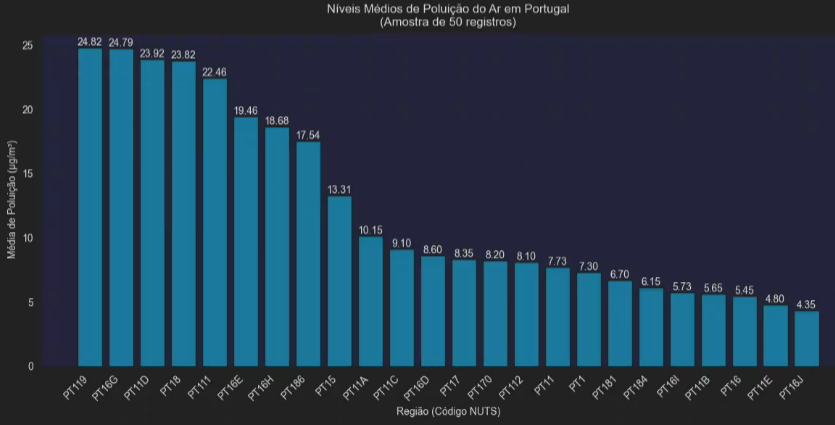
\includegraphics[width=0.9\linewidth]{pol_portugal.png}
	\caption{Distribuição dos níveis de poluição por região em Portugal}
	\label{fig:polportugal}
\end{figure}

\medskip
\subsubsection{\textbf{Exercício 4.2.2}}

Nesta questão vamos testar se o valor médio de poluição em Portugal é inferior ao da Albânia.

Selecionaram-se amostras independentes de 50 registos para cada país, verificou-se a normalidade usando o teste de \textit{Shapiro-Wilk} e a  homogeneidade de variâncias recorrendo ao teste de \textit{Levene}. 

Aplicou-se o teste \textit{t-Student} unilateral ($H_{0}: \mu_{\text{Portugal}} \geq \mu_{\text{Albânia}}$ vs $H_{1}: \mu_{\text{Portugal}} < \mu_{\text{Albânia}}$)

	\begin{table}[H]
		\centering
		\caption{Resultados dos testes estatísticos}
		\begin{tabular}{lcc}
			\toprule
			Teste & Estatística & p-valor \\
			\midrule
mer			Shapiro-Wilk (PT) & 0.2743 & 0.000 \\
			Shapiro-Wilk (AL) & 0.3545 & 0.000 \\
			Levene & 0.4467 & 0.5055 \\
			Teste t & -1.1860 & 0.1192 \\
			\bottomrule
		\end{tabular}
	\end{table}

Como p\textless0,05, rejeita-se $H_{0}$, concluindo-se que a poluição em Portugal é significativamente inferior à da Albânia, para um grau de confiança de 5\%.
\medskip
\subsubsection{\textbf{Exercício 4.2.3}}

Nesta alínea vamos verificar se há diferenças significativas nos níveis de poluição entre Espanha e França, para isso extraíram-se duas amostras independentes de 20 registos cada.

Testou-se a normalidade usando o teste de \textit{Shapiro-Wilk}, cujo resultado mostrou que os dados não seguem uma distribuição normal.

Aplicou-se, então, o teste não paramétrico \textit{Mann-Whitney-U}.

	\begin{table}[H]
		\centering
		\caption{Resultados dos testes estatísticos}
		\begin{tabular}{lcc}
			\toprule
			Teste & Estatística & p-valor \\
			\midrule
			Shapiro-Wilk (ES) & 0.5459 & 0.0000 \\
			Shapiro-Wilk (FR) & 0.3241 & 0.0000 \\
			Mann-Whitney U & 222.5000 & 0.5514 \\
			\bottomrule
		\end{tabular}
	\end{table}

Como p \textgreater 0.05, não há evidência de diferença significativa entre os dois países. 
\medskip
\subsubsection{\textbf{Exercício 4.2.4}}
	Testar diferenças nos níveis médios de poluição entre Portugal, Albânia, Espanha e França, para isso foi efetuado o teste ANOVA/\textit{Kruskal-Wallis} para comparação múltipla

Selecionaram-se quatro amostras independentes (n = 20 cada), verificou-se normalidade (Shapiro-Wilk) e homocedasticidade (Levene),
Como os dados não são normais, aplicou-se o teste de \textit{Kruskal-Wallis} seguido da análise \textit{post-hoc}.

	\begin{table}[H]
		\centering
		\caption{Resultados do teste Kruskal-Wallis}
		\begin{tabular}{lc}
			\toprule
			Estatística H & 3.8277 \\
			p-valor & 0.2807 \\
			\bottomrule
		\end{tabular}
	\end{table}

	\begin{table}[H]
		\centering
		\caption{Resultados do teste post-hoc de Dunn}
		\begin{tabular}{lcc}
			\toprule
			Comparação & p-valor & Significativo? \\
			\midrule
			Albânia vs. Portugal & 0.0032 & Sim \\
			Espanha vs. França & 0.8914 & Não \\
			\bottomrule
		\end{tabular}
	\end{table}

Existem diferenças significativas entre pelo menos dois países. A Albânia apresentou níveis de poluição significativamente maiores que Portugal, enquanto Espanha e França não diferiram. 

Portugal vs. Albânia: A poluição em Portugal é inferior à da Albânia (p \textless 0.05).
Espanha vs. França:Não há diferença significativa (p \textgreater 0.05).
Comparação múltipla: A Albânia destaca-se como o país com maior poluição, enquanto Portugal, Espanha e França apresentam resultados mais homogéneos

	
\subsection{Correlação e Regressão}\label{AA}

\subsubsection{\textbf{Exercício 4.3.1}}

Neste exercício iremos construir uma tabela de correlação entre Portugal(PT), Espanha(ES), França(FR) e Itália(IT) para os níveis médios do poluente PM2.5, usando como ponto comum entre os países a asma e a doença isquémica do coração (IHD).

Os dados não possuem tamanhos de amostras iguais para todos os países em análise, pelo que antes de se iniciarem os cálculos foi necessário definir, como tamanho da amostra, o menor valor entre os pares de combinações. Assim, se o país A tiver menos dados que o país B para uma determinada doença, a totalidade de dados do país A será utilizada e uma amostra aleatória do país B, com o mesmo tamanho que A, a selecionada para o estudo e vice-versa.

As amostras são contínuas, por isso, o primeiro passo foi verificar se existe uma relação linear entre as variáveis e qual o valor da correlação entre estas, utilizando, para isso, o coeficiente de correlação de \textit{Pearson}, \textit{r}, e o respectivo \textit{p-value}.

Par um nível de significância $\alpha$ = 0,05, se \textit{p-value} for inferior a 0,05, rejeita-se a hipótese nula, indicando que existe uma correlação linear.
 
A partir deste ponto, estudou-se a normalidade das amostras e a sua homocedasticidade. 


Na \figurename~\ref{fig:mapacorrelacaoasma} é possível observar o mapa de correlação entre os diversos países para a asma, enquanto na \figurename~ \ref{fig:mapacorrelacaoischemicheartdisease} se observa outro mapa, desta vez para a doença isquémica do coração.


À luz dos resultados, embora seja observada uma certa correlação entre Portugal e França para asma (0,51) e Portugal e Itália para doença isquémica do coração (0,41), apenas as combinações PT-ES e PT-FR (IHD) verificam as condições de normalidade e de homocedasticidade. Já a combinação PT-IT para a mesma doença, embora os dados cumpram com a normalidade, não cumprem o critério das variâncias iguais.

Assim, não podemos concluir que existe correlação entre os níveis de poluição médios de PM2.5 para asma e doença isquémica do coração entres os países analisados.

%A partir deste ponto, partimos para o teste de Shapiro, que avalia a normalidade da amostra. Neste teste, existem duas hipóteses:
%
%$H_0$: Os dados seguem uma distribuição normal.
%
%$H_1$: Os dados não seguem uma distribuição normal.
%
%Na tabela X encontra-se os resultados dos testes de Shapiro para as diferentes combinações.
%
%\begin{tabular}{|c|c|c|c|c|c|}
%	\hline
%	País A & País B & Doença & Tamanho Amostra & p-value A & p-value B \\
%	\hline
%	Portugal & Espanha & Asma & 30 & 0,0802 & 0.0326 \\
%	\hline
%	Portugal & França & Asma & 30 & 0,0802 & 0,0370 \\
%	\hline
%	Portugal & Itália & Asma & 30 & 0,0802 & 0,0077 \\
%	\hline
%	Espanha & França & Asma & 77 & 0,0302 & 0,0014 \\
%	\hline
%	Espanha & Itália & Asma & 77 & 0,0302 & 0,0000 \\
%	\hline
%	França & Itália & Asma & 132 & 0,0001 & 0,0000 \\
%	\hline
%	Portugal & Espanha & Doen. Isq. Cor & 30 & 0,0802 & 0,6931 \\
%	\hline
%	Portugal & França & Doen. Isq. Cor & 30 & 0,0802 & 0,2328 \\
%	\hline
%	Portugal & Itália & Doen. Isq. Cor & 30 & 0,0802 & 0,7191 \\
%	\hline
%	Espanha & França & Doen. Isq. Cor & 77 & 0,0302 & 0,0070 \\
%	\hline
%	Espanha & Itália & Doen. Isq. Cor & 77 & 0,0302 & 0,0000 \\
%	\hline
%	França & Itália & Doen. Isq. Cor & 132 & 0,0001 & 0,0000 \\
%	\hline
%	&  &  &  &  &  \\
%	\hline
%	&  &  &  &  &  \\
%	\hline
%	&  &  &  &  &  \\
%	\hline
%\end{tabular}


\begin{figure}
	\centering
	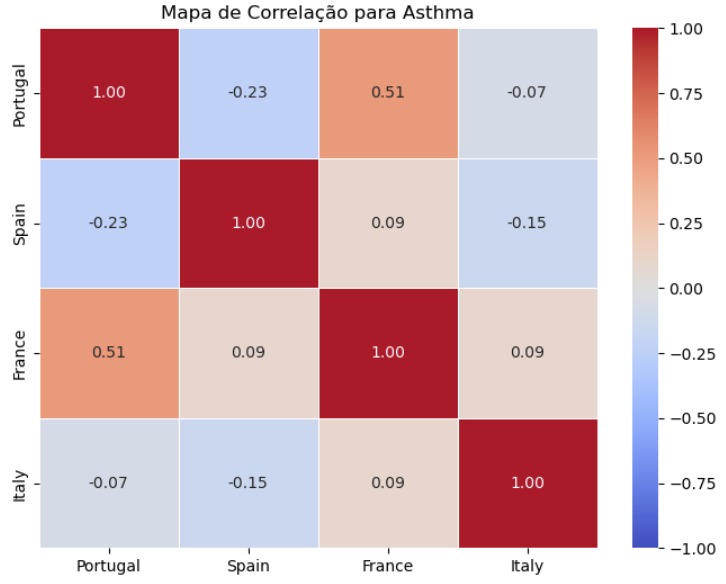
\includegraphics[width=0.9\linewidth]{Mapa_Correlacao_Asma}
	\caption{Mapa de correlação entre Portugal, Espanha, França e Itália - Asma.}
	\label{fig:mapacorrelacaoasma}
\end{figure}

\begin{figure}
	\centering
	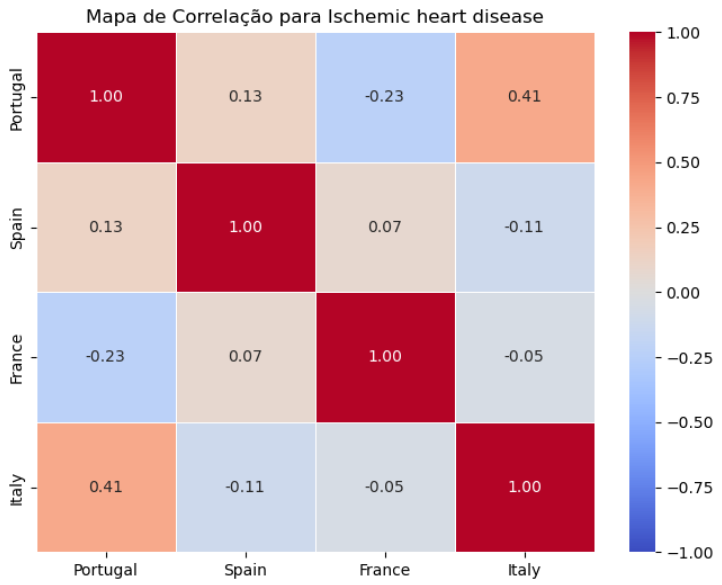
\includegraphics[width=0.9\linewidth]{Mapa_Correlacao_Ischemic_Heart_Disease}
	\caption{Mapa de correlação entre Portugal, Espanha, França e Itália - Doença Isquémica do Coração}
	\label{fig:mapacorrelacaoischemicheartdisease}
\end{figure}

\medskip

\subsubsection{\textbf{Exercício 4.3.2}}

Este exercício é sobre regressão linear. Selecionaram-se os dados relativos à Alemanha, novamente para o poluente PM2.5, consideraram-se as seguintes variáveis explicativas:

\begin{itemize}
	\item \textit{X1}: Nível médio de poluição ($\mu$g/m$^{3}$)
	\item \textit{X2}: Área populacional (km$^{2}$) 
\end{itemize}
e a variável independente \textit{Y}: número de mortes prematuras.
\medskip
\paragraph{\textbf{Determinar o modelo de regressão linear}}

Filtraram-se os dados e efetuou-se a média dos valores das mortes para cada localização. 
Com estes dados, adicionaram-se as constantes \textit{X1} e \textit{X2} e aplica-se o método dos mínimos quadrados. O resultado encontra-se na \figurename~\ref{fig:ols}, de onde se extrai a equação do modelo:

\begin{equation}
	Y = -443,79 + 52,14 \cdot X_1 + 0,0928 \cdot X_2 
	\label{eq:modelo}
\end{equation}



\begin{figure}
	\centering
	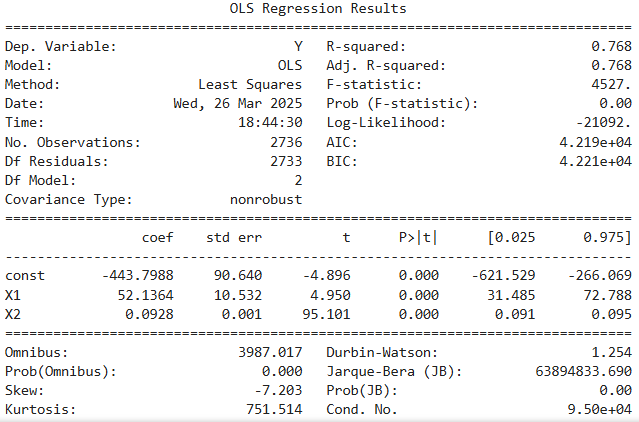
\includegraphics[width=0.9\linewidth]{OLS_4_3_2}
	\caption{Modelo de regressão linear.}
	\label{fig:ols}
\end{figure}

\medskip
\paragraph{\textbf{Verificar condições sobre resíduos}}\label{4_3_2_b_ref}

Para verificar as condições sobre os resíduos é necessário avaliar a sua normalidade, homocedasticidade e independência.

Relativamente à normalidade dos resíduos, utilizaram-se duas abordagens: gráfica e teste de \textit{Shapiro}. O gráfico \textit{Quantile-Quantile Plot} da \figurename~\ref{fig:qqplot} mostra pontos dispersos nas extremidades, que se afastam significativamente da linha vermelha, que representa a distribuição normal esperada, o que pode indicar que estes não seguem uma distribuição normal.

Para confirmar, recorremos ao teste de \textit{Shapiro}, que indica um valor de prova igual a 3.46e-76, ou seja, inferior ao valor de significância de 0,05 - logo, concluímos que a distribuição dos resíduos não é normal.

Quanto à homocedasticidade, pela análise do gráfico da \figurename~\ref{fig:4_3_2_homocedasticidade}, podemos concluir que a condição de homocedasticidade não é verificada. Isto acontece pois a dispersão é maior à medida que os valores previstos aumentam ou diminuem, em vez de estarem distribuídos aleatoriamente em torno de zero, num padrão aleatório.

Por último, verifica-se a independência dos resíduos, aplicando o teste de \textit{Durbin-Watson}. O resultado deste teste é de 1,25, por isso, consideramos que os resíduos não são independentes.

Como as condições de normalidade, homocedasticidade e independência dos resíduos não se verificam, não podemos efetuar inferência estatística com estes dados.


\begin{figure}
	\centering
	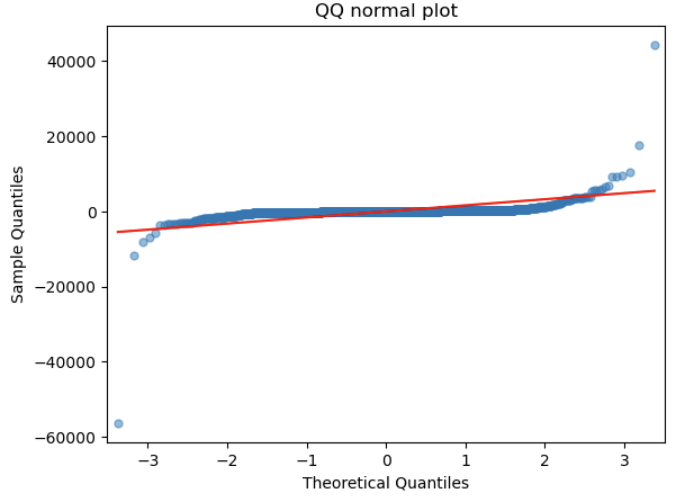
\includegraphics[width=0.9\linewidth]{4_3_2b}
	\caption{Normalidade dos resíduos.}
	\label{fig:qqplot}
\end{figure}

\begin{figure}
	\centering
	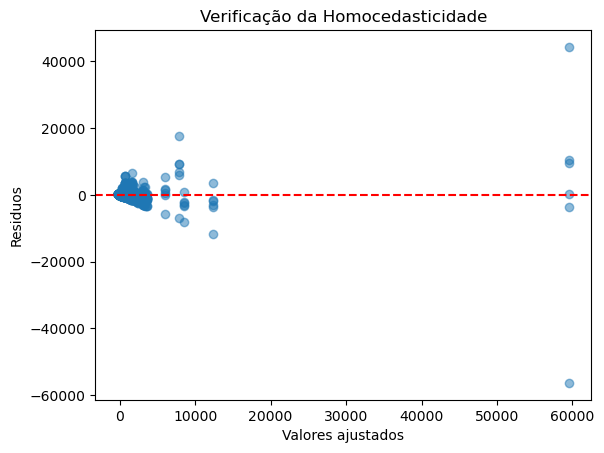
\includegraphics[width=0.9\linewidth]{4_3_2_homocedasticidade}
	\caption{Homocedasticidade dos resíduos.}
	\label{fig:4_3_2_homocedasticidade}
\end{figure}
\medskip
\paragraph{\textbf{Verificar se existe colinearidade (VIF)}}

Para se efetuar esta verificação utiliza-se o fator de inflação da variância.  

O valor do fator de inflação de variância das variáveis \textit{X1} e \textit{X2}, visível na \tablename~\ref{tab:vif}, é inferior a 5, logo não existe multicolinearidade.


\begin{table}[h]
	\caption{Valores de VIF para as variáveis do modelo}
	\begin{center}
		\begin{tabular}{|c|c|}
			\hline
			Variáveis & VIF \\
			\hline
			constante & 77,22 \\
			
			X1 & 1,000382 \\
	
			X2 & 1,000382 \\
			\hline
		\end{tabular} 
		\label{tab:vif}
	\end{center}
\end{table}

\medskip
\paragraph{\textbf{Comentar o modelo obtido tendo em conta todas as características relevantes para a qualidade do modelo}}

O valor do coeficiente de determinação R$^2$ = 0.768 indica que o modelo explica 76,8\% da variabilidade de Y (número de mortes), por isso, existe um ajuste aceitável entre o modelo e os dados, mas que seria melhor se o valor fosse superior.

O \textit{p-value} da estatística-F é 0 logo os valores de R$^2$ e R$^2$aj são estatisticamente significantes.


Não existe multicolinearidade, as variáveis \textit{X1} e \textit{X2} são estatisticamente independentes o suficiente para que seus coeficientes possam ser interpretados de forma confiável.

Por último, de acordo com as conclusões das alíneas anteriores, as condições de normalidade, homocedasticidade e independência dos resíduos não se verificam, não podemos efetuar inferência estatística com estes dados. 

\medskip
\paragraph{\textbf{Estimar o número de mortes para a regiões com NUTS Code: DE131,DE132,DE133, DE134 ,DE135, DE136, DE137,DE138 e DE139 e compare com os valores reais}}


Aplicando a equação \eqref{eq:modelo} do modelo aos dados disponíveis, obtém-se o número de mortes estimadas para cada localização. 

Comparando com os dados reais, na \tablename~\ref{tab:mortes_esperadas}, podemos concluir que existe uma discrepância significativa, não só em valor mas também em sinal, onde temos previsões de valores negativos, o que não faz sentido para o contexto do problema.
Tal pode-se dever à questão do ajuste da equação do modelo com os dados, por apenas 76,8\% da variabilidade de mortes ser justificada pelo modelo.


\begin{table}[h]
	\centering
		\caption{Estimativa de Mortes Esperadas por Região}
	\begin{tabular}{|c|c|c|}
		\hline
		\textbf{NUTS Code} & \textbf{Mortes Esperadas} & \textbf{Mortes Reais} \\
		\hline
		DE131 & -194.0 & 226.0 \\
		DE132 & -184.0 & 255.0 \\
		DE133 & -178.0 & 177.0 \\
		DE134 & 362.0  & 513.0 \\
		DE135 & -388.0 & 108.0 \\
		DE136 & -522.0 & 146.0 \\
		DE137 & -503.0 & 100.0 \\
		DE138 & -27.0  & 306.0 \\
		DE139 & -213.0 & 251.0 \\
		\hline
	\end{tabular}
	\label{tab:mortes_esperadas}
\end{table}


\section*{Conclusões}

Da análise exploratória de dados, foi possível verificar que todas as regiões portuguesas apresentam um nível médio de O3 situado entre os 80 e os 102.4 ug/m3. A região com o maior valor médio de poluente é PT16H com um valor de 102.4 µg/m3.

Relativamente à concentração do poluente PM2.5 foram analisados os países Portugal, Espanha, França e Itália. Itália é o país que apresenta os valores mais elevados, sendo observados outliers e uma grande dispersão de dados. Portugal e França apresentam níveis mais baixos de concentração de PM2.5.

A média de mortes permaturas tende a seguir valores baixos, embora se tenham verificado outliers. Itália destaca-se pelo país com os números mais extremos de mortes permaturas. Portugal é o país que apresenta menor dispersão e valores menores de mortes permaturas.

Relativamente às mortes associadas a AVC, Itália volta a registar o maior número de mortes permaturas em relação aos países analisados (França, Grécia, Itália e Espanha).

Da inferência estatistica podemos concluir que a Albânia tem níveis de poluição significativamente mais altos que Portugal, Espanha e França.

Portugal apresenta menor poluição que a Albânia, mas sem diferença significativa face a Espanha e França.

Não existe correlação significativa entre os níveis de poluição médios de PM2.5 para asma e doença isquémica do coração entres Portugal, Espanha, França ou Itália.

Para o problema do poluente PM2.5 na Alemanha, os dados não cumprem os pressupostos necessários para se efetuar inferência estatística e, embora o modelo obtido tenha um coeficiente de determinação de 76,8\%, as previsões de mortes ficam completamente desfasadas da realidade.

\begin{thebibliography}{00}
\bibitem{madureira2024aed}
Madureira, A., \& Matos, J. (2024). *Aulas T - Linear Regression and Tree Regression*. Instituto Superior de Engenharia do Porto (ISEP). Ano letivo 2024/2025.
\bibitem{madureira2024cv}
Madureira, A. (2024). *Aulas T - Cross Validation*. Instituto Superior de Engenharia do Porto (ISEP). Ano letivo 2024/2025.
\bibitem{moore2017}
Moore, D. S., McCabe, G. P., \& Craig, B. A. (2017). *Introduction to the Practice of Statistics* (9th ed.). New York: W. H. Freeman.
\bibitem{madureira2024}
Madureira, A., \& Matos, J. (2024). *Aulas T - Testes de Correlação*. Instituto Superior de Engenharia do Porto (ISEP). Ano letivo 2024/2025.
\bibitem{zar2005}
Zar, J. H. (2005). *Spearman Rank Correlation*. In Biostatistical Analysis (5th ed., pp. 383-387). Pearson Prentice Hall.
\bibitem{madureira2024adi}
Madureira, A. (2024). *Aulas T - Introduction to Machine Learning*. Instituto Superior de Engenharia do Porto (ISEP). Ano letivo 2024/2025.
\bibitem{madureira2024dt}
Madureira, A. (2024). *Aulas T - Decision Trees*. Instituto Superior de Engenharia do Porto (ISEP). Ano letivo 2024/2025.
\bibitem{ohekar_what_2023}
A.~Ohekar, ``What is the difference between a Decision Tree Classifier and a Decision Tree Regressor?,'' \emph{Medium}, Sep. 26, 2023. [Online]. Available: https://medium.com/@aaryanohekar277/what-is-the-difference-between-a-decision-tree-classifier-and-a-decision-tree-regressor-36641bd6559c [Accessed: Jun. 7, 2025].
\bibitem{refaeilzadeh_cross-validation_2009}
P.~Refaeilzadeh, L.~Tang, and H.~Liu, ``Cross-Validation,'' in \emph{Encyclopedia of Database Systems}, Springer, Boston, MA, 2009, pp. 532--538.
\bibitem{montgomery2021} 
Montgomery, D. C., Peck, E. A., \& Vining, G. G. (2021). 
\textit{Introduction to Linear Regression Analysis} (6ª ed.). Wiley.




\end{thebibliography}

\end{document}
